\chapter{Patching}

Patching is \textbf{slow} and \textbf{expensive}.
This is due to many factors:
first of all there's the need to run \textbf{regression} tests, to check correctness of standard behaviour and of he bug to be corrected;
besides, new behaviours and problems may arise because of the new code;
in case of a complex problem requiring $N$ patches,
the \textbf{scheduling} of such patches must be taken into account;
in general is advised to patch using an automated process exploiting patching agents and environment.

\subsection{Common Vulnerability Scoring System}

Note that, for instance, \textit{Industrial Control Systems} \textbf{cannot be patched}, because it would imply for the production to be \textit{suspended} and for the whole system to be \textit{certified} again.\\
This forces an admin to decide whether \textit{"to-patch or not to-patch"}.\\
About this matter a \textbf{Common Vulnerability Scoring System} (\textit{CVSS}) has been developed.
Its aim is to consider the main features of a vulnerability and compute a score based upon them;
in the initial idea such score should have allowed to define a score threshold to decide whether to patch or not.
However, such idea doesn't work for two main reasons:
\begin{enumerate}
    \item Single vulnerabilities are not of interest, while \textit{intrusions} are i.e. chaining and exploiting multiple vulnerabilities
    \item \textit{CVSS} totally \textit{ignores} the \textbf{system}, but the context in this topic is fundamental 
\end{enumerate}
Even if it cannot be helpful as a guide for an admin to perform the above mentioned decision, it can be truly instructive to understand how impactful a vulnerability can be, 
and it can provide an approximation of how \textit{difficult} may be for an attacker to exploit such vulnerability.
The CVSS provides three \textit{metrics} to evaluate vulnerabilities risks:
\begin{itemize}
    \item \textbf{Base} fundamental characteristics constant over time and user environments.
    Such metric aims to provide an intuitive and clear vulnerability representation.
    \item \textbf{Temporal} the characteristics that change over time but not among user environments
    \item \textbf{Metric} the characteristics relevant and unique to a particular user environment
    \begin{itemize}
        \item \textit{Access Vector} (network/adjacent/local/physical)
        \item \textit{Attack complexity}
        \item Required \textit{privileges} and \textit{user interaction}
        \item \textit{Scope}: whether the attack enables to reach resouces that are controlled by another entity, i.e. beyond the scope of the vulnerable component
        \item \textit{Temporal Score}: whether the exploit exists, only a proof-of-concept exists, or if is unknown.
    \end{itemize}
\end{itemize}

\subsection{CVSS revisions}
\textit{Dragos} in 2022 proposed a revision of scores in the CVSS considering the attacker point of view, claiming to have better ones,
but still raising up many doubts.

Later on the same experts team created the \textbf{EPSS} as a measure of exploitability:
it is a \textit{Neural-Network} based system which \ul{estimates the probability that a vulnerability will be exploited}.
It is unclear on which data the AI has been trained, accuracy, tuning, etc...
EPSS does not consider risk, context or whatsoever, it's just a probability estimator.

\textbf{SSVC} \textit{Stakeholder-Specific Vulnerability Categorization} aims specifically to produce an \textbf{action} for the defendant to perform regarding a vulnerability. 
Imagine a decision tree 5 levels deep. An admin must make 5 "decisions"\footnote{In the sense of answering 5 questions} about a vulnerability, and then a leaf of the tree can be one among 4:
\begin{enumerate}
    \item {\color{green}Track}
    \item {\color{yellow}Track}
    \item {\color{orange}Attend}
    \item {\color{red}Act}
\end{enumerate}

Considering the decisions to be made by the admin:
\begin{enumerate}
    \item \textbf{State of Exploitation}
    \begin{itemize}
        \item \textit{None}: No evidence of atcive exploitation and no public \textit{Proof of Concept} (PoC) on how to exploit the vulnerability
        \item \textbf{Public PoC} Sites like ExploitDB or Metasploit contain PoC on such vulnerability $v$ or $v$ has a well-known method of exploitation 
        \item \textbf{Active} Credible sources claim that $v$ is shared, observable and has been exploited in the past.
    \end{itemize}
    \item \textbf{Technical Impact}
    \begin{itemize}
        \item \textbf{Partial} control of the software given to the attacker e.g. DoS attack
        \item \textbf{Total} control of the software or total information disclosure given to the attacker.
    \end{itemize}
    \item \textbf{Automatable}
    \item \textbf{Mission Prevalence \& Public Well Being}
    \begin{itemize}
        \item Does the vulnerable component provide support for the (attacker?) mission? Is it essential? Is it not so useful?
        \item Which kind and how much harm the attack may cause and if it is irreversibile or not.
        Physical, psychological, financial, environmental 
    \end{itemize}
    \item \textbf{Mitigation}
    \note{This is not included in the decision tree!}
    \begin{itemize}
        \item Fix available/unavailable
        \item System change difficulty
        \item Actual Fix or Workaround
    \end{itemize}
\end{enumerate}

\begin{figure}
    \centering
    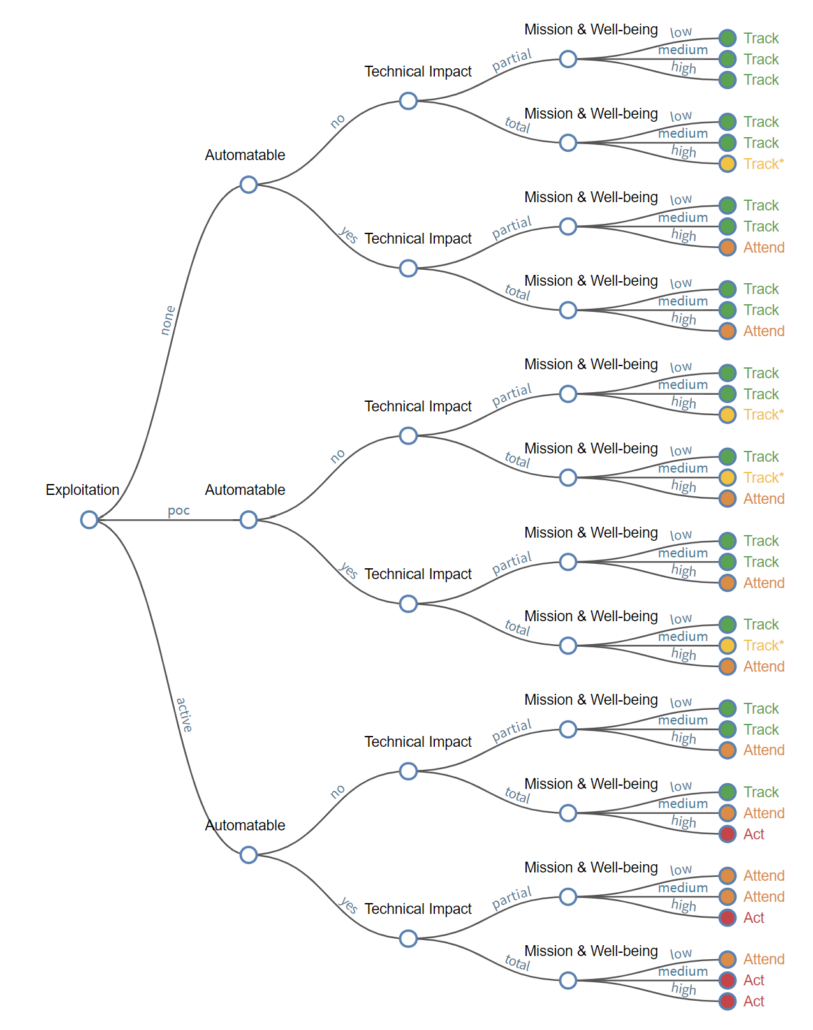
\includegraphics[width=0.7\textwidth]{images/cisa_ssvc_tree.png}
    \caption{SSVC Decision tree}
    \label{fig:cisa_ssvc_tree}
\end{figure}